\section{Thực nghiệm: đo chuẩn gradient theo độ sâu tại bước khởi tạo}
\label{sec:thucnghiem}

Mục~\ref{sec:nguyennhan} chỉ cho một \emph{chặn trên} \eqref{eq:governing}. Mục
này đo giá trị thực của gradient để thấy chặn đó chặt đến đâu, và kiểm tra khi
nào tầng đầu thực sự không còn được cập nhật. Chỉ một cặp (hàm kích hoạt, sơ đồ
khởi tạo) thay đổi giữa hai điều kiện; mọi thứ khác giữ nguyên.

\subsection{Giao thức}

\begin{itemize}[leftmargin=*, itemsep=2pt]
  \item \textbf{Kiến trúc.} $L$ tầng tuyến tính: $L-1$ tầng ẩn rộng $D=64$ và
    một tầng ra một chiều; đầu vào $64$ chiều. Hàm kích hoạt đặt sau mỗi tầng ẩn,
    không đặt sau tầng ra. Mọi độ lệch khởi tạo bằng $0$.
  \item \textbf{Độ sâu.} $L \in \{5,\ 10,\ 20\}$.
  \item \textbf{Điều kiện A} --- sigmoid, khởi tạo
    \texttt{nn.init.xavier\_normal\_}~\cite{GlorotBengio2010},
    $\operatorname{Var}(w) = 2/(n_{\text{in}}+n_{\text{out}})$.
  \item \textbf{Điều kiện B} --- ReLU, khởi tạo
    \texttt{nn.init.kaiming\_normal\_(nonlinearity='relu')}~\cite{He2015},
    $\operatorname{Var}(w) = 2/n_{\text{in}}$.
    Cả $L$ tầng (kể cả tầng ra) dùng cùng sơ đồ khởi tạo của điều kiện.
  \item \textbf{Dữ liệu và mất mát.} $N=256$ mẫu,
    $\mathbf{x}\sim\mathcal{N}(\mathbf{0},\mathbf{I}_{64})$,
    $y\sim\mathcal{N}(0,1)$; \texttt{nn.MSELoss()} (trung bình trên lô).
  \item \textbf{Hạt giống.} $\{42,\ 100,\ 2024,\ 2026,\ 9999\}$. Với mỗi hạt giống,
    \texttt{random}, \texttt{numpy} và \texttt{torch} được đặt lại, dữ liệu được
    sinh \emph{trước}, rồi mới khởi tạo mạng --- nên A và B thấy cùng một lô dữ
    liệu. \texttt{torch.use\_deterministic\_algorithms(True)}, \texttt{float32},
    CPU.
  \item \textbf{Phép đo.} Đo tại bước khởi tạo, một lượt lan truyền tiến và
    \emph{một} lượt lan truyền ngược duy nhất; không có bước tối ưu nào.
\end{itemize}

\paragraph{Chuẩn gradient.} Với $\mathbf{g}^{[l]} = \partial\mathcal{L}/\partial\mathbf{W}^{[l]}$
(chỉ trọng số, không tính độ lệch),
\[
  \left\|\mathbf{g}^{[l]}\right\|_F \;=\; \sqrt{\textstyle\sum_{i,j}\left(g^{[l]}_{ij}\right)^{2}}
  \qquad(\texttt{torch.linalg.norm(W.grad)}),
  \qquad
  \rho \;=\; \frac{\left\|\mathbf{g}^{[1]}\right\|_F}{\left\|\mathbf{g}^{[L]}\right\|_F}.
\]
Chặn $c$ trong bảng được \emph{đo}, không giả định:
$c = \max\sigma'\cdot\overline{\sigma_{\max}}$, với $\overline{\sigma_{\max}}$ là
trung bình chuẩn phổ của $\mathbf{W}^{[2]},\dots,\mathbf{W}^{[L]}$ --- các ma trận
mà lượt ngược thực sự đi qua.

\paragraph{Tiêu chí đóng băng.} So chuẩn tuyệt đối $\left\|\mathbf{g}^{[1]}\right\|_F$
với epsilon máy là sai tiêu chí: phép cộng \texttt{float32} $w - \eta g$ bị làm
tròn về đúng $w$ khi $\left|\eta g\right|$ nhỏ hơn khoảng nửa ulp của $w$, tức
một đại lượng \emph{tương đối} so với $|w|$. Vì vậy ta đo, với $\eta = 0.1$,
\[
  r \;=\; \frac{\eta\left\|\mathbf{g}^{[1]}\right\|_F}{\left\|\mathbf{W}^{[1]}\right\|_F}
  \quad\text{so với}\quad
  \epsilon_{32} = 2^{-23} \approx 1.19\times10^{-7},
\]
và kiểm tra trực tiếp: tỉ lệ phần tử của $\mathbf{W}^{[1]}$ không đổi sau phép
trừ $\mathbf{W}^{[1]} - \eta\,\mathbf{g}^{[1]}$, cùng với
\texttt{torch.equal} (toàn bộ cập nhật bị mất).

\tcbinputlisting{%
  enhanced, breakable,
  colback=gray!10, colframe=aivnGreen, coltitle=white, colbacktitle=aivnGreen,
  title={Thực nghiệm đo gradient với PyTorch (\texttt{experiment.py})},
  fonttitle=\bfseries\sffamily,
  listing only, listing engine=listings,
  listing file={experiment.py},
  listing options={%
    language=Python,
    basicstyle=\ttfamily\footnotesize,
    commentstyle=\color{ForestGreen},
    keywordstyle=\color{blue},
    stringstyle=\color{red!70!black},
    numbers=left, numberstyle=\tiny\color{gray}, numbersep=5pt,
    breaklines=true, showstringspaces=false,
    xleftmargin=1.5em, framexleftmargin=1.5em,
    upquote=true, columns=fullflexible, keepspaces=true,
    mathescape=false, texcl=false,
  }%
}

\subsection{Kết quả}

Hai bảng dưới chép nguyên từ \texttt{results.md} do \texttt{experiment.py} sinh
ra (PyTorch 2.14.0+cpu, CPython 3.12.3): trung bình $\pm$ độ lệch chuẩn mẫu
(\texttt{ddof=1}) trên $5$ hạt giống, ba chữ số có nghĩa. Chạy lại script cho
kết quả trùng từng byte.

\begin{table}[H]
\centering
\small
\renewcommand{\arraystretch}{1.2}
\begin{tabular}{@{}rccccc@{}}
\toprule
$L$ & $c$ (chặn) & $\left\|\mathbf{g}^{[1]}\right\|_F$ & $\left\|\mathbf{g}^{[L]}\right\|_F$
  & $\rho$ & $\log_{10}\rho$ \\
\midrule
\multicolumn{6}{@{}l}{\textit{A: sigmoid + Xavier}} \\
$5$  & $0.449\pm0.00761$ & $(3.96\pm1.15)\times10^{-3}$  & $3\pm2.16$    & $(2.18\pm1.75)\times10^{-3}$  & $-2.78\pm0.358$ \\
$10$ & $0.469\pm0.00277$ & $(2.79\pm0.523)\times10^{-6}$ & $4.93\pm2.48$ & $(9.25\pm10.1)\times10^{-7}$  & $-6.19\pm0.373$ \\
$20$ & $0.479\pm0.00293$ & $(1.59\pm0.62)\times10^{-12}$ & $8.44\pm3.2$  & $(2.28\pm1.63)\times10^{-13}$ & $-12.7\pm0.29$ \\
\midrule
\multicolumn{6}{@{}l}{\textit{B: ReLU + He}} \\
$5$  & $2.4\pm0.0379$  & $1.93\pm0.75$  & $10.9\pm4.48$ & $0.189\pm0.0584$ & $-0.74\pm0.135$ \\
$10$ & $2.59\pm0.0179$ & $1.4\pm0.571$  & $9.55\pm9.71$ & $0.302\pm0.25$   & $-0.638\pm0.358$ \\
$20$ & $2.68\pm0.0141$ & $4.08\pm7.49$  & $28.7\pm57.6$ & $0.462\pm0.581$  & $-0.53\pm0.409$ \\
\bottomrule
\end{tabular}
\begin{captionbelowboxaivn}
Bảng 3: Chặn $c$ đo được và chuẩn gradient tại bước khởi tạo, trung bình $\pm$ độ
lệch chuẩn trên $5$ hạt giống.
\end{captionbelowboxaivn}
\end{table}

\begin{table}[H]
\centering
\small
\renewcommand{\arraystretch}{1.2}
\begin{tabular}{@{}rcccc@{}}
\toprule
$L$ & $r = \eta\|\mathbf{g}^{[1]}\|_F/\|\mathbf{W}^{[1]}\|_F$ & $r/\epsilon_{32}$
  & \makecell{Tỉ lệ phần tử\\ $\mathbf{W}^{[1]}$ không đổi} & \makecell{Đóng băng\\ hoàn toàn} \\
\midrule
\multicolumn{5}{@{}l}{\textit{A: sigmoid + Xavier}} \\
$5$  & $(4.93\pm1.45)\times10^{-5}$   & $413\pm122$                  & $0.00176\pm0.00087$ & $0/5$ \\
$10$ & $(3.46\pm0.638)\times10^{-8}$  & $0.291\pm0.0535$             & $0.678\pm0.0553$    & $0/5$ \\
$20$ & $(1.98\pm0.764)\times10^{-14}$ & $(1.66\pm0.641)\times10^{-7}$ & $1\pm0$            & $5/5$ \\
\midrule
\multicolumn{5}{@{}l}{\textit{B: ReLU + He}} \\
$5$  & $0.017\pm0.00666$  & $(1.42\pm0.558)\times10^{5}$ & $0\pm0$ & $0/5$ \\
$10$ & $0.0123\pm0.00505$ & $(1.03\pm0.424)\times10^{5}$ & $0\pm0$ & $0/5$ \\
$20$ & $0.0361\pm0.0663$  & $(3.02\pm5.56)\times10^{5}$  & $0\pm0$ & $0/5$ \\
\bottomrule
\end{tabular}
\begin{captionbelowboxaivn}
Bảng 4: Tiêu chí đóng băng tầng $1$ với $\eta = 0.1$. Cột cuối đếm số hạt giống
mà \texttt{torch.equal} xác nhận toàn bộ cập nhật bị làm tròn mất.
\end{captionbelowboxaivn}
\end{table}

\subsection{Phân tích}

\textbf{Điều kiện A (sigmoid + Xavier).} $\log_{10}\rho$ giảm gần tuyến tính theo
độ sâu: $-2.78$, $-6.19$, $-12.7$ ở $L = 5, 10, 20$. Quy về mỗi tầng,
$10^{\log_{10}\rho/(L-1)}$ cho $0.202$, $0.205$, $0.215$ --- một hệ số suy giảm
gần như không đổi, tức suy giảm theo hàm mũ đúng như chặn dự báo khi $c<1$.

Tuy nhiên chặn đo được là $c \approx 0.45$--$0.48$, \emph{không phải} $0.25$:
chuẩn phổ trung bình của các ma trận Xavier trong mạng, $c/0.25$, là khoảng
$1.8$--$1.9$ chứ không bằng $1$.
Hệ số suy giảm thực ($\approx0.2$) còn nhỏ hơn $c$ khoảng hai lần; khoảng cách
đó chính là hai yếu tố (a) bão hoà và (b) lệch hướng kỳ dị mà $c$ bỏ qua. Nói
cách khác, ở đây chặn đúng nhưng lỏng. (Vì
$\mathbf{g}^{[l]}$ còn chứa thừa số kích hoạt $\mathbf{a}^{[l-1]}$, phép so sánh
giữa $\rho$ và $c^{\,L-1}$ chỉ có ý nghĩa ở bậc độ lớn.)

\textbf{Đóng băng ở điều kiện A phụ thuộc độ sâu, và chỉ xảy ra hoàn toàn ở
$L=20$.} Với $L=5$, $r/\epsilon_{32} = 413$: tầng $1$ được cập nhật bình thường.
Với $L=10$, $r/\epsilon_{32} = 0.291 < 1$, nhưng chỉ $67.8\%$ phần tử của
$\mathbf{W}^{[1]}$ đứng yên và \emph{không} hạt giống nào đóng băng hoàn toàn:
$r$ là trung bình trên cả ma trận, còn phép làm tròn xảy ra từng phần tử, nên các
phần tử có $|g_{ij}|/|w_{ij}|$ lớn vẫn nhích được. Tầng $1$ ở $L=10$ bị đóng
băng \emph{một phần}. Chỉ ở $L=20$ ($r/\epsilon_{32}\approx1.66\times10^{-7}$)
toàn bộ cập nhật bị làm tròn mất, ở cả $5/5$ hạt giống. Vì $r$ tỉ lệ thuận với
$\eta$, tốc độ học nhỏ hơn $0.1$ sẽ đẩy ngưỡng này xuống độ sâu nhỏ hơn.

\textbf{Điều kiện B (ReLU + He).} Chặn đo được là $c \approx 2.4$--$2.68 > 1$,
vậy mà không có bùng nổ: $\rho$ trung bình nằm trong $[0.189,\ 0.462]$, dưới
$1$. Đây là minh hoạ trực tiếp cho điểm đã nêu ở Mục~\ref{sec:nguyennhan}:
$c>1$ chỉ cho phép bùng nổ, không bảo đảm nó. Điều He bảo toàn là
\emph{phương sai} tín hiệu (độ lợi trung bình bình phương $\approx1$), không
phải $\sigma_{\max}$. Tầng $1$ không đóng băng ở bất kỳ độ sâu nào
($r/\epsilon_{32}\sim10^{5}$, không phần tử nào đứng yên).

Điều mà một lần chạy đơn lẻ không cho thấy là \textbf{độ phân tán tăng theo độ
sâu}: độ lệch chuẩn của $\log_{10}\rho$ tăng từ $0.135$ ($L=5$) lên $0.409$
($L=20$), và ở $L=20$ độ lệch chuẩn của $\left\|\mathbf{g}^{[1]}\right\|_F$
($7.49$) lớn hơn cả trung bình ($4.08$) --- phân phối lệch mạnh, bị một vài hạt
giống chi phối. Khởi tạo đúng giữ \emph{bậc độ lớn trung bình}, nhưng không giữ
được từng lần khởi tạo; đó là lý do cần báo cáo trung bình $\pm$ độ lệch chuẩn
thay vì một con số.

\begin{figure}[H]
\centering
\begin{tikzpicture}
\begin{axis}[
    width=0.80\linewidth, height=6.0cm,
    xlabel={Độ sâu $L$},
    ylabel={$\log_{10}\rho$ (trung bình $\pm$ độ lệch chuẩn)},
    xtick={5,10,20}, xmin=3, xmax=22,
    ymin=-14, ymax=1,
    axis lines=left,
    legend style={font=\scriptsize, at={(0.03,0.03)}, anchor=south west, draw=none, fill=none},
    tick label style={font=\scriptsize},
    label style={font=\scriptsize},
    grid=major, grid style={gray!20},
]
\addplot[thick, aivnGreen, mark=*, mark size=1.6pt,
         error bars/.cd, y dir=both, y explicit] coordinates {
  (5,-2.78) +- (0,0.358) (10,-6.19) +- (0,0.373) (20,-12.7) +- (0,0.29)
};
\addlegendentry{A: sigmoid + Xavier}
\addplot[thick, brandIndigo, mark=square*, mark size=1.5pt,
         error bars/.cd, y dir=both, y explicit] coordinates {
  (5,-0.74) +- (0,0.135) (10,-0.638) +- (0,0.358) (20,-0.53) +- (0,0.409)
};
\addlegendentry{B: ReLU + He}
\end{axis}
\end{tikzpicture}

\begin{figurecaptionmodern}
\capfig{$\log_{10}\rho$ theo độ sâu, số liệu của Bảng~3. Điều kiện A giảm gần
tuyến tính theo $L$ (suy giảm hàm mũ, $\approx0.2$ mỗi tầng); điều kiện B nằm
gần $0$ nhưng thanh sai số rộng dần theo $L$.\label{fig:gradnorm}}
\end{figurecaptionmodern}
\end{figure}

\begin{guidelinebox}{Cách đọc một bảng chuẩn gradient khi gỡ lỗi mô hình thật}
Khi một mô hình sâu không giảm được mất mát huấn luyện, hãy in chuẩn gradient
theo tầng, trên vài hạt giống, \emph{trước khi} chỉnh tốc độ học hay thêm dữ liệu:
\begin{itemize}[leftmargin=*, itemsep=1pt]
  \item \textbf{Giảm đơn điệu nhiều bậc độ lớn về phía đầu vào} $\Rightarrow$
    nhiều khả năng là triệt tiêu gradient. Kiểm tra hàm kích hoạt và sơ đồ khởi
    tạo trước tiên.
  \item \textbf{Tăng đơn điệu, hoặc xuất hiện \texttt{inf}/\texttt{NaN}}
    $\Rightarrow$ bùng nổ gradient. Cắt ngưỡng gradient, giảm tốc độ
    học~\cite{Pascanu2013}.
  \item \textbf{Mọi tầng cùng bậc độ lớn} $\Rightarrow$ đường truyền gradient
    không phải nút thắt; nên tìm nguyên nhân ở chỗ khác (tốc độ học, dữ liệu,
    hàm mất mát).
  \item \textbf{Chuẩn bằng đúng $0$ ở nhiều tầng với ReLU} $\Rightarrow$ hiện
    tượng ``ReLU chết''; cân nhắc LeakyReLU hoặc GELU.
\end{itemize}
Để biết tầng đầu có thực sự đứng yên hay không, đừng so chuẩn gradient với
epsilon máy; hãy tính $r = \eta\|\mathbf{g}^{[1]}\|_F/\|\mathbf{W}^{[1]}\|_F$ và
đếm số phần tử không đổi sau một bước cập nhật, như Bảng~4.
\end{guidelinebox}

\begin{notebox}
Thực nghiệm đo gradient tại \emph{bước khởi tạo}, chưa huấn luyện. Điều này là cố
ý: nó tách biệt ảnh hưởng của kiến trúc và khởi tạo khỏi động lực học. Kết quả
vì thế không nói gì về việc gradient thay đổi ra sao sau nhiều bước tối ưu;
một mạng bắt đầu ở trạng thái đóng băng hoàn toàn (như điều kiện A, $L=20$) chỉ
thoát ra được nếu các tầng phía sau thay đổi đủ để nâng $r$ lên trên
$\epsilon_{32}$.
\end{notebox}

\subsection{Động lực học trong quá trình huấn luyện: PlainNet so với ResNet}
\label{sec:training-dynamics}

Các mục trước chỉ đo tại bước khởi tạo. Mục này theo dõi cùng các đại lượng
\emph{trong suốt} $10$ epoch huấn luyện, và đặt residual connection cạnh mạng
thuần để kiểm tra ba câu hỏi: (a) residual connection có cứu được sigmoid không;
(b) ReLU + residual connection không có BatchNorm có ổn định không; (c) ở độ
sâu lớn, BatchNorm cộng identity path chuyển thành độ chính xác ra sao.

\paragraph{Thiết lập.} Dữ liệu là CIFAR-10: $10{,}000$ ảnh huấn luyện (tập con
cố định bằng hạt giống $0$), đánh giá trên toàn bộ $10{,}000$ ảnh test, chuẩn hoá
theo kênh rồi duỗi thành vector $3072$ chiều. Mạng là MLP rộng $256$: tầng
\emph{stem} \texttt{Linear(3072, 256)} $\to$ Norm $\to$ Act, rồi $L$ tầng ẩn
\texttt{Linear(256, 256)}, rồi tầng \emph{head} \texttt{Linear(256, 10)}.
PlainNet xếp $L$ khối \texttt{Linear}$\to$Norm$\to$Act; ResNet xếp $L/2$ khối
\[
  \mathbf{x}_{l+1} = \phi\big(\mathbf{x}_l + F(\mathbf{x}_l)\big),\qquad
  F = \texttt{Linear}\to\text{Norm}\to\phi\to\texttt{Linear}\to\text{Norm},
\]
tức activation $\phi$ đặt \emph{sau} phép cộng (post-addition), và cả hai kiến
trúc có đúng $L+2$ ma trận trọng số. Norm là \texttt{BatchNorm1d} hoặc
\texttt{Identity} (khi có BatchNorm thì \texttt{bias=False}). Lưới thí nghiệm:
$2$ kiến trúc $\times$ $L\in\{8,16,32\}$ $\times$ $4$ biến thể
\{Sigmoid + Xavier, Sigmoid + Xavier + BN, ReLU + Kaiming, ReLU + Kaiming + BN\}
$\times$ $3$ hạt giống $\{42, 100, 2024\}$ $=72$ lần chạy. Tối ưu bằng SGD,
$\eta=0.1$, không momentum, không weight decay, batch $128$, $10$ epoch,
\texttt{float32} trên CPU với \texttt{torch.use\_deterministic\_algorithms(True)}.
Một lần chạy được coi là \emph{phân kỳ} khi mất mát huấn luyện không còn hữu hạn;
lần chạy đó dừng ngay.

\paragraph{Phép đo.} Một \emph{probe batch} cố định gồm $512$ ảnh huấn luyện
được đưa qua một lượt forward/backward riêng (chế độ train, không có bước tối
ưu, buffer BatchNorm được khôi phục) tại epoch $0$ (khởi tạo) và sau mỗi epoch.
Với $\mathbf{g}_{\text{stem}} = \partial\mathcal{L}/\partial\mathbf{W}_{\text{stem}}$
và $\mathbf{g}_{\text{head}} = \partial\mathcal{L}/\partial\mathbf{W}_{\text{head}}$
trên probe batch,
\[
  \text{stem gnorm} \;=\; \left\|\mathbf{g}_{\text{stem}}\right\|_F,
  \qquad
  \rho \;=\; \frac{\left\|\mathbf{g}_{\text{stem}}\right\|_F}{\left\|\mathbf{g}_{\text{head}}\right\|_F}.
\]
Ngoài ra, ở mỗi bước huấn luyện ta ghi cập nhật tương đối thực sự của stem,
$r = \|\mathbf{W}_{t+1}-\mathbf{W}_t\|_F/\|\mathbf{W}_t\|_F$, và báo cáo trung vị
theo epoch dưới dạng $r/\epsilon_{32}$. Mọi số liệu dưới đây là trung bình
$\pm$ độ lệch chuẩn mẫu (\texttt{ddof=1}) trên $3$ hạt giống, lấy từ
\texttt{results\_training.json}.

% Tables in this document are numbered by hand; the counter is set only so
% that \ref{tab:training-dynamics} resolves to the printed number.
\setcounter{table}{4}
\begin{table}[htbp]
\centering
\footnotesize
\renewcommand{\arraystretch}{1.2}
\begin{adjustbox}{max width=\linewidth}
\begin{tabular}{@{}rcccccc@{}}
\toprule
& \multicolumn{2}{c}{Test acc (\%)} & \multicolumn{2}{c}{$\log_{10}\rho$}
& \multicolumn{2}{c}{Stem gnorm $\left\|\mathbf{g}_{\text{stem}}\right\|_F$} \\
\cmidrule(lr){2-3}\cmidrule(lr){4-5}\cmidrule(l){6-7}
Epoch & PlainNet & ResNet & PlainNet & ResNet & PlainNet & ResNet \\
\midrule
\multicolumn{7}{@{}l}{\textit{ReLU + Kaiming + BatchNorm}} \\
$0$  & $10.6\pm0.962$ & $10.0\pm0.052$ & $2.81\pm0.0832$   & $0.348\pm0.101$   & $626\pm59.4$          & $45.0\pm1.39$ \\
$1$  & $13.1\pm0.649$ & $18.3\pm4.03$  & $-1.30\pm0.0419$  & $-0.914\pm0.0523$ & $0.0735\pm0.00931$    & $0.701\pm0.0672$ \\
$5$  & $17.7\pm0.396$ & $25.8\pm4.31$  & $-1.36\pm0.154$   & $-0.569\pm0.145$  & $0.0531\pm0.00477$    & $0.993\pm0.401$ \\
$10$ & $22.9\pm1.09$  & $32.0\pm5.77$  & $-1.26\pm0.145$   & $-0.342\pm0.156$  & $0.0469\pm0.0076$     & $1.07\pm0.221$ \\
\midrule
\multicolumn{7}{@{}l}{\textit{ReLU + Kaiming, không BatchNorm}} \\
$0$  & $9.94\pm0.0954$ & $9.58\pm0.37$ & $-0.133\pm0.191$ & $-0.737\pm0.0462$ & $2.95\pm0.9$ & $(2.32\pm0.244)\times10^{3}$ \\
$1$  & $11.5\pm2.57^{\dagger}$  & div.$^{\ast}$ & $0.221\pm0.317^{\dagger}$  & div.$^{\ast}$ & $0.589\pm0.423^{\dagger}$ & div.$^{\ast}$ \\
$5$  & $18.9\pm0.0354^{\dagger}$ & div.$^{\ast}$ & $0.384\pm0.0145^{\dagger}$ & div.$^{\ast}$ & $0.891\pm0.503^{\dagger}$ & div.$^{\ast}$ \\
$10$ & $16.1\pm6.82^{\dagger}$  & div.$^{\ast}$ & $0.0497\pm0.545^{\dagger}$ & div.$^{\ast}$ & $5.41\pm3.08^{\dagger}$   & div.$^{\ast}$ \\
\bottomrule
\end{tabular}
\end{adjustbox}

\smallskip
\begin{minipage}{\linewidth}\scriptsize
$^{\ast}$\,div.: $3/3$ hạt giống phân kỳ ngay ở epoch $1$, bước $1$.
$^{\dagger}$\,Trung bình trên $2$ hạt giống: hạt giống $42$ của PlainNet phân kỳ ở
epoch $1$, bước $3$. Toàn lưới có $10/72$ lần chạy phân kỳ ($9$ ResNet ReLU không
BN ở cả ba độ sâu, $1$ PlainNet ReLU không BN, $L=32$); không lần chạy nào có
BatchNorm hoặc sigmoid bị phân kỳ.
\end{minipage}

\begin{captionbelowboxaivn}
\refstepcounter{table}\label{tab:training-dynamics}%
Bảng~\thetable: Động lực học ở $L=32$, ReLU + Kaiming, có và không có BatchNorm:
độ chính xác test, $\log_{10}\rho$ và stem gnorm trên probe batch, trung bình
$\pm$ độ lệch chuẩn trên $3$ hạt giống.
\end{captionbelowboxaivn}
\end{table}

\begin{figure}[htbp]
\centering
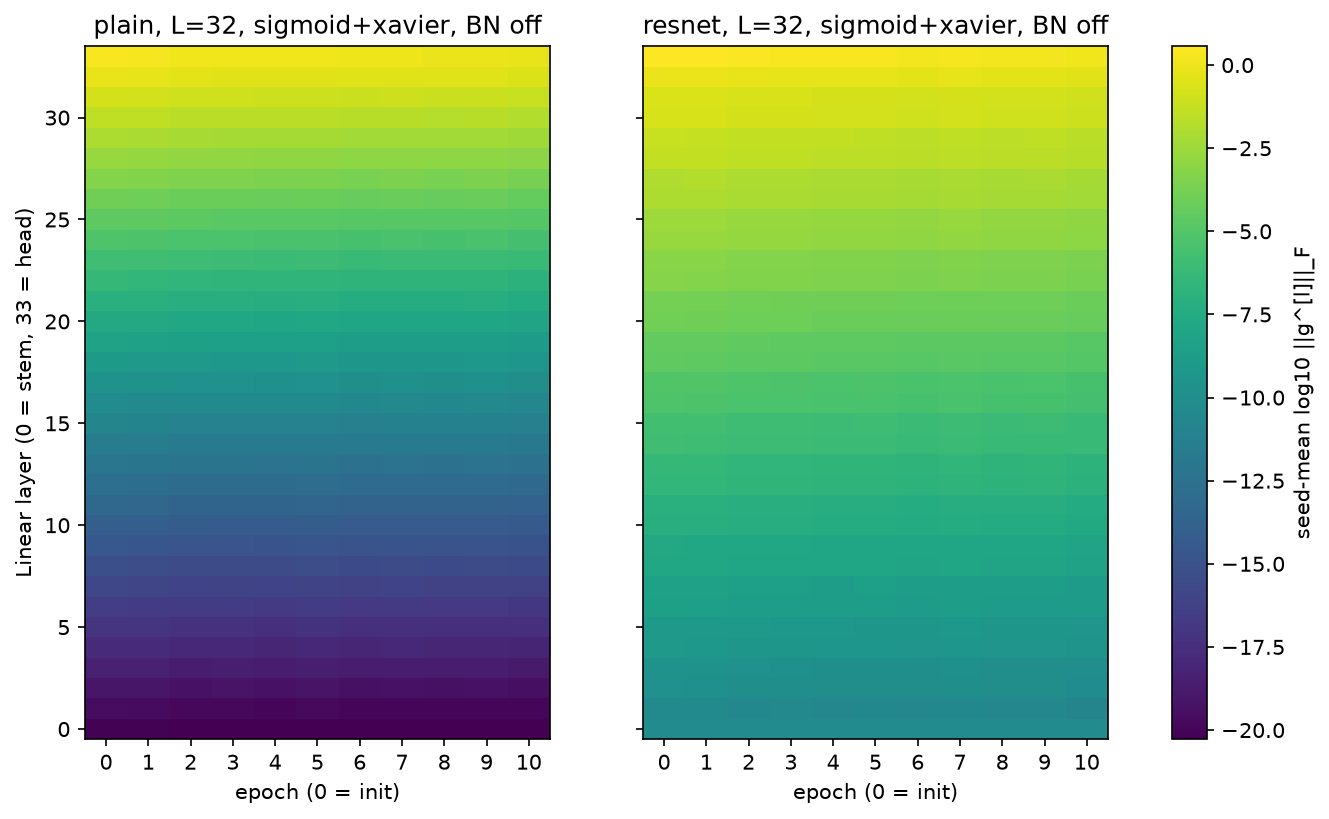
\includegraphics[width=\linewidth]{figures/heatmap_plain_vs_resnet.png}
\begin{figurecaptionmodern}
\capfig{Heatmap của $\log_{10}\left\|\mathbf{g}^{[l]}\right\|_F$ (trung bình trên
$3$ hạt giống, thang màu viridis chung cho hai panel, từ khoảng $-20$ đến $0$)
ở $L=32$, Sigmoid + Xavier, không BatchNorm. Trục hoành: epoch ($0$ = khởi tạo);
trục tung: chỉ số tầng tuyến tính ($0$ = stem, $33$ = head). Trái: PlainNet;
phải: ResNet. Kết luận: residual connection kéo stem từ khoảng $10^{-20.5}$
lên khoảng $10^{-10.8}$, nhưng gradient vẫn giảm theo hàm mũ từ head về stem
và không epoch nào thay đổi được điều đó.\label{fig:heatmap-plain-resnet}}
\end{figurecaptionmodern}
\end{figure}

\begin{figure}[htbp]
\centering
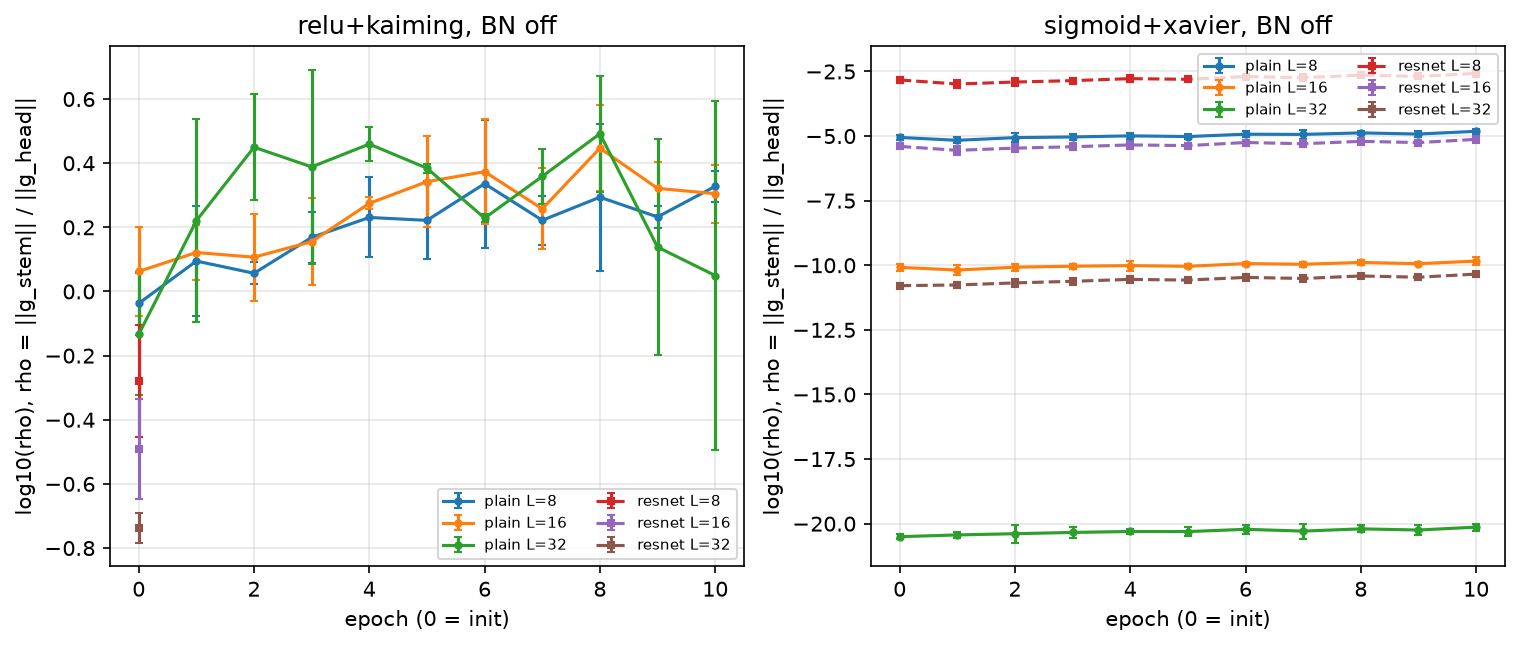
\includegraphics[width=\linewidth]{figures/gradient_flow_residual.png}
\begin{figurecaptionmodern}
\capfig{$\log_{10}\rho$ theo epoch ($0$ = khởi tạo), không BatchNorm; đường liền
là PlainNet, đường đứt là ResNet, mỗi màu một độ sâu $L\in\{8,16,32\}$, thanh
sai số là độ lệch chuẩn trên các hạt giống còn hữu hạn. Trái: ReLU + Kaiming;
phải: Sigmoid + Xavier. Kết luận: với sigmoid, mọi đường gần như nằm ngang suốt
$10$ epoch, nên huấn luyện không tự sửa được vanishing gradient; với ReLU,
ResNet không BN chỉ có điểm epoch $0$ vì mọi lần chạy đều phân kỳ ở epoch
$1$.\label{fig:gradflow-residual}}
\end{figurecaptionmodern}
\end{figure}

\paragraph{(a) Sigmoid ResNet với activation sau phép cộng vẫn vanishing.}
\emph{Cơ chế.} Đặt $\mathbf{s}_l = \mathbf{x}_l + F(\mathbf{x}_l)$. Jacobian
của một khối là
\[
  \frac{\partial\mathbf{x}_{l+1}}{\partial\mathbf{x}_l}
  \;=\; \operatorname{diag}\!\big(\sigma'(\mathbf{s}_l)\big)
        \left(\mathbf{I} + \frac{\partial F}{\partial\mathbf{x}_l}\right),
  \qquad \sigma'(\cdot)\le\tfrac14 .
\]
Identity path chỉ bảo vệ gradient \emph{bên trong} dấu ngoặc. Thừa số
$\operatorname{diag}(\sigma')$ nằm ngoài nên vẫn bị nhân một lần mỗi khối, và
chặn~\eqref{eq:governing} của Mục~\ref{sec:nguyennhan} vẫn áp dụng, chỉ với số
thừa số ít hơn. Trên đường ngắn nhất từ head về stem, PlainNet đi qua $L+1$
thừa số $\sigma'$ (stem cộng $L$ tầng ẩn), còn ResNet đi qua $L/2+1$ (stem cộng
$L/2$ activation sau phép cộng). Lý thuyết vì vậy dự báo
$\log_{10}\rho_{\text{ResNet}}/\log_{10}\rho_{\text{Plain}}\approx(L/2+1)/(L+1)$.

\emph{Bằng chứng.} Tại khởi tạo, $\log_{10}\rho$ của PlainNet là $-5.05$,
$-10.1$, $-20.5$ và của ResNet là $-2.83$, $-5.40$, $-10.8$ ở $L=8,16,32$. Tỉ
số đo được $0.560$, $0.536$, $0.526$ khớp với dự báo $5/9=0.556$,
$9/17=0.529$, $17/33=0.515$. Quy về mỗi thừa số $\sigma'$, hệ số suy giảm là
$0.23$--$0.27$, sát chặn $1/4$, ở cả hai kiến trúc.
Hình~\ref{fig:heatmap-plain-resnet} cho thấy trường gradient theo tầng không đổi
qua $10$ epoch, và Hình~\ref{fig:gradflow-residual} (phải) cho thấy
$\log_{10}\rho$ chỉ nhích $0.24$--$0.45$ sau $10$ epoch. Ở $L=32$, cập nhật
tương đối của stem ResNet chỉ còn $r/\epsilon_{32}\approx0.8\text{--}2.3\times10^{-8}$
(PlainNet: đúng $0$, mọi bước đều bị \texttt{torch.equal} xác nhận không đổi).
Độ chính xác test của cả $18$ lần chạy Sigmoid không BN ($6$ cấu hình) ở epoch $10$ đều là
$10.0\%$, tức mức đoán ngẫu nhiên.

\emph{Kết luận.} Residual connection chia đôi số mũ của vanishing gradient
nhưng không xoá nó; muốn identity path thực sự là đường cao tốc, activation
bão hoà phải nằm \emph{trong} nhánh $F$, không đặt sau phép cộng.

\paragraph{(b) ReLU ResNet không BatchNorm phân kỳ ngay epoch đầu.}
\emph{Cơ chế.} Không có BatchNorm, nhánh $F$ với khởi tạo Kaiming giữ phương sai
của đầu vào thay vì triệt tiêu nó, và phép cộng của identity path cộng dồn
phương sai qua từng khối:
\[
  \operatorname{Var}(\mathbf{x}_{l+1}) \;\approx\;
  \operatorname{Var}(\mathbf{x}_l) + \operatorname{Var}\big(F(\mathbf{x}_l)\big)
  \;=\; (1+\kappa)\operatorname{Var}(\mathbf{x}_l)
  \;\Longrightarrow\;
  \operatorname{Var}(\mathbf{x}_{L/2}) \approx (1+\kappa)^{L/2}\operatorname{Var}(\mathbf{x}_0),
\]
với $\kappa=\operatorname{Var}(F(\mathbf{x}_l))/\operatorname{Var}(\mathbf{x}_l)$
cỡ $1$. Phương sai của forward pass tăng theo hàm mũ của số khối, kéo theo
logits và gradient. PlainNet + Kaiming nhân phương sai với khoảng $1$ mỗi tầng
nên không cộng dồn.

\emph{Bằng chứng.} Phương sai forward không được đo trực tiếp, nhưng
$\mathbf{g}_{\text{head}} = \boldsymbol{\delta}_{\text{out}}\mathbf{a}^{\top}$ tỉ
lệ với độ lớn activation cuối. Tại khởi tạo, $\|\mathbf{g}_{\text{head}}\|_F$ của
ResNet là $51.8$, $313$, $1.26\times10^{4}$ ở $L=8,16,32$ ($4$, $8$, $16$ khối),
tức tăng khoảng $1.57$--$1.59$ lần mỗi khối về chuẩn, hay khoảng $2.5$ lần về
phương sai. PlainNet cùng cấu hình giữ ở $2.4$--$4.3$. Mất mát trên probe batch
lúc khởi tạo của ResNet là $9.90$, $41.8$, $1480$, so với $\ln 10\approx2.30$ của
một bộ phân loại ngẫu nhiên. Stem gnorm ở $L=32$ là $(2.32\pm0.244)\times10^{3}$
(Bảng~\ref{tab:training-dynamics}), nên bước SGD đầu tiên có
$\eta\|\mathbf{g}_{\text{stem}}\|_F\approx232$. Kết quả là $9/9$ lần chạy phân kỳ
ở epoch $1$, và mạng càng sâu thì càng sớm: bước $3$--$4$ ($L=8$), bước $2$
($L=16$), bước $1$ ($L=32$). Trong Hình~\ref{fig:gradflow-residual} (trái), các
đường ResNet chỉ còn điểm epoch $0$. PlainNet ReLU không BN cũng không hoàn toàn
an toàn: $1/3$ hạt giống ở $L=32$ phân kỳ (epoch $1$, bước $3$).

\emph{Kết luận.} Identity path chuyển phép \emph{nhân} của mạng thuần thành phép
\emph{cộng} của phương sai; không có cơ chế chuẩn hoá, phép cộng đó tự nó cộng
dồn thành bùng nổ.

\paragraph{(c) Ở $L=32$, BatchNorm + identity path giữ $\rho$ gần $1$ và
chuyển thành độ chính xác.}
\emph{Cơ chế.} BatchNorm ở cuối nhánh $F$ ép
$\operatorname{Var}(F(\mathbf{x}_l))\approx1$ bất kể $l$ (với $\gamma=1$,
$\beta=0$ lúc khởi tạo), nên phương trình ở (b) đổi từ nhân sang cộng:
\[
  \operatorname{Var}(\mathbf{x}_{l+1}) \approx \operatorname{Var}(\mathbf{x}_l) + 1
  \;\Longrightarrow\;
  \operatorname{Var}(\mathbf{x}_l) \approx \operatorname{Var}(\mathbf{x}_0) + l .
\]
Phương sai tăng tuyến tính chứ không theo hàm mũ, và tỉ trọng của nhánh $F$
so với identity path giảm cỡ $1/\sqrt{l}$. Vì vậy mỗi thừa số
$\mathbf{I}+\partial F/\partial\mathbf{x}_l$ gần $\mathbf{I}$, và tích của chúng
không trôi theo hàm mũ. PlainNet + BN không có identity path, nên gradient đi về
stem phải qua $L+1=33$ cặp BN--ReLU nối tiếp và không có gì giữ chúng gần
nhau.

\emph{Bằng chứng (Bảng~\ref{tab:training-dynamics}, phần trên).}
\begin{itemize}[leftmargin=*, itemsep=1pt]
  \item \textbf{$\rho$ của ResNet ở gần $1$.} Qua $11$ lần đo, $\log_{10}\rho$
    trung bình của ResNet nằm trong $[-0.914,\ 0.348]$, tức $\rho\in[0.122,\ 2.23]$.
    PlainNet bùng nổ về phía stem lúc khởi tạo ($\log_{10}\rho=2.81$,
    $\rho\approx643$, stem gnorm $626$), rồi rơi xuống $-1.30$ sau epoch $1$ và
    ở lại quanh $-1.2$ đến $-1.4$ ($\rho\approx0.05$).
  \item \textbf{Stem của ResNet được cập nhật mạnh hơn nhiều.} Ở epoch $10$,
    stem gnorm là $1.07\pm0.221$ (ResNet) so với $0.0469\pm0.0076$ (PlainNet),
    và cập nhật tương đối $r/\epsilon_{32}$ là $(5.08\pm0.46)\times10^{4}$ so với
    $423\pm76.4$, tức stem của ResNet học nhanh hơn khoảng $120$ lần.
  \item \textbf{Độ chính xác tương ứng.} Test acc ở epoch $10$ là
    $32.0\pm5.77\%$ (ResNet) so với $22.9\pm1.09\%$ (PlainNet). Theo từng hạt
    giống, ResNet đạt $38.5$, $29.9$, $27.5\%$ và PlainNet đạt $24.2$, $22.5$,
    $22.2\%$, nên mọi hạt giống ResNet đều vượt mọi hạt giống PlainNet.
\end{itemize}
Lợi thế này chỉ xuất hiện ở độ sâu lớn. Ở $L=8$ và $L=16$, PlainNet + BN nhỉnh
hơn ($35.1\pm4.10$ so với $31.6\pm5.72\%$; $29.5\pm2.88$ so với $28.2\pm6.75\%$).
Độ chính xác của PlainNet giảm đơn điệu theo $L$ ($35.1\to29.5\to22.9\%$), còn
ResNet gần như giữ nguyên ($31.6\to28.2\to32.0\%$).

\emph{Kết luận.} BatchNorm chặn sự cộng dồn phương sai, identity path giữ đường
gradient về stem; cần \emph{cả hai} thì stem mới học được ở $L=32$, và đó là
nguồn của khoảng cách $9$ điểm phần trăm.

\begin{notebox}
Số liệu chỉ có $3$ hạt giống và $10$ epoch trên $10{,}000$ ảnh, nên các khoảng
$\pm$ của ResNet ($4$--$7$ điểm phần trăm) còn rộng. Hai biến thể Sigmoid + BN
không được đưa vào Bảng~\ref{tab:training-dynamics}; ở $L=32$, chúng đạt
$18.9\pm3.55\%$ (PlainNet) và $22.3\pm6.47\%$ (ResNet) ở epoch $10$, với
$\log_{10}\rho$ trung bình của cả hai ở trong $[-0.41,\ 0.09]$ suốt quá trình huấn luyện.
BatchNorm một mình đã xoá vanishing gradient của sigmoid về mặt chuẩn gradient,
nhưng không đưa độ chính xác lên ngang ReLU + BN.
\end{notebox}
